\chapter{Implementation in seL4}
\label{chap:implementation}

In the previous chapter we presented our mechanisms for temporal isolation and safe resource sharing
in a high-assurance microkernel. 
Now we delve into the implementation details of scheduling contexts, scheduling context donation,
timeout fault handlers, and IPC forwarding in \selfour.

First we survey new and changed kernel objects, followed by the updated system call API, and ...
\TODO{update when done}.

\section{Objects}

We add two new objects to the kernel, \emph{\glspl{SCO}} and \emph{resume objects}. Additionally, we modify
the \gls{TCB} object although do not increase its total size. Finally, we modify the notification
object to allow \glspl{SCO} to allow single-threaded, passive servers to receive signals in
addition to IPC messages.

\subsection{Resume objects}
\label{s:resume}

Resume objects, modelled after KeyKOS~\citep{Bomberger_FFHLS_92}, are
a new object type that generalise
``reply capabilities'' of baseline \selfour introduced in \cref{s:ipc}.
Recall that in baseline \selfour, the receiver of the message (i.e.\ the
server) receives the reply capability in a magic ``reply slot'' in its
capability space. The server replies by invoking that
capability. Resume objects remove the magic by explicitly representing
the reply channel, and servers with multiple clients can dedicate a resume object per client.
Instead of generating a one-shot reply capability in a reply slot on a \call, the operation
populates a resume object, while \recv de-populates the resume object. 
They also
provide more efficient support for stateful servers that handle
concurrent client sessions, which we expand on further when we introduce the changed system call \gls{API} in \cref{s:new-api}.

Resume objects are small (16 bytes on 32-bit platforms, and 32 bytes on 64-bit platforms), and
contain the fields shown in \cref{tab:reply_object}.

\begin{table}[h]
    \centering
    \rowcolors{2}{gray!25}{}
    \begin{tabularx}{\textwidth}{lX}\toprule
        \emph{Field} & \emph{Description} \\\midrule
        \code{tcb}    & The calling or waiting thread that is blocked on this reply object. \\
        \code{prev} & \code{NULL} if this is the start of the call stack, otherwise points to the previous
        reply object in the call stack. \\
        \code{next} & Either a pointer to the scheduling context that was last donated using this
        reply object, if this reply object is the head of a call stack (the last caller before the
        server) or a pointer to the next reply object in the stack. 0 if no scheduling context was
        passed along the stack.\\\bottomrule
    \end{tabularx}
    \caption{Fields in a reply object.}
    \label{tab:reply_object}
\end{table}

There are three states a resume object can be in: idle, meaning it is not currently being used,
waiting, meaning it is being used by a thread blocked and waiting for a message, or active,
which means the resume object currently has a thread blocked waiting for a reply associated with it.

\begin{figure}[h]
    \centering
    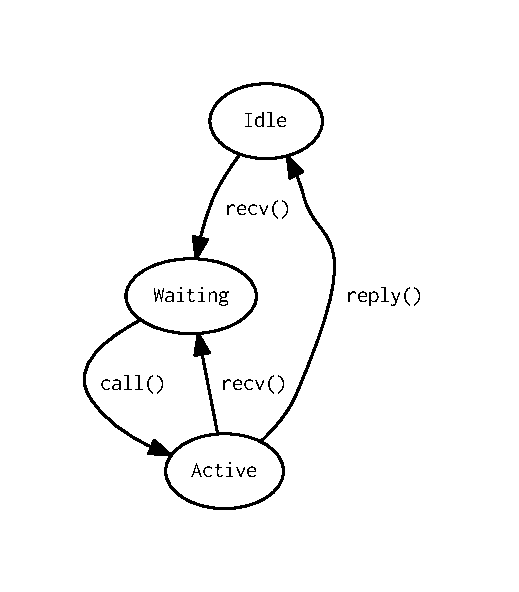
\includegraphics[width=0.6\textwidth]{resume}
    \caption{State diagram of resume objects.}
    \label{f:resume-state-diagram}
\end{figure}

Valid state transitions are shown in \cref{f:resume-state-diagram}. Resume objects are provided to
\code{recv} system calls along with endpoint capabilities, which transitions them from idle to
waiting.
If the endpoint is invoked with a \code{call}, the caller is blocked on the resume capability, and
it transitions to active.  
If a resume object is directly invoked, using a sending system call (recall from
\cref{sec:sel4-system-call-and-invocations} that sending system calls are \code{send},
\code{nbsend}, \code{call}, \code{reply}) then a reply message is delivered to the thread blocked on
the resume object. If a resume object is in an active state, and provided to \code{recv}, the object
is first invoked, and removed from the call stack, which we now examine in detail. 

\subsubsection{The call stack}

Active resume objects track the \emph{call stack} that is built as nested \call operations take
place. A \call triggers to a push operation, adding to the top of the stack, and a reply message a
pop, removing the top of the stack.  The call stack allows us to track the path of a donated
scheduling context, from caller to callee, so that it can be returned to the previous caller
regardless of which thread sends the reply message. This is a direct consequence of flexible resume
capabilities: resume capability can be moved between threads, and \emph{any} thread can execute the
reply: usually the server, but occasionally a timeout fault handler, or a nested server which
received the resume capability via \gls{IPC} forwarding. It is therefore impossible to derive the
original callee from the thread sending the reply message.

The call stack is structured as a doubly-linked list, with one minor difference: the head of the
call stack is the scheduling context that was donated along the stack, which itself contains a
pointer to the thread currently executing on it. Each resume object then forms a node in the
stack, going back to the original caller at the base. The \gls{SCO} remains the head of the stack
until the \gls{SCO} returns to the initial caller and the stack is fully dismantled.  When a reply
message is sent, the scheduling context travels back along the call stack and the head resume object
is popped.  Reply objects also point to the thread which donated the \gls{SCO} along the stack,
allowing the SCO to be returned to that thread when a reply message is sent.  This process is
illustrated in in \cref{f:reply-stack}, where $A$ has called $S_{1}$ which has called  $S_{2}$.

\begin{figure}
    \centering
    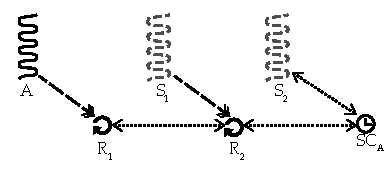
\includegraphics[width=0.7\textwidth]{replychain}
    \caption{The state of the reply stack when a nested server $S_{2}$ is
performing a request on behalf of an initial server $S_{1}$ for client $A$.}
    \label{f:reply-stack}
\end{figure}

In a capability system, one of the biggest challenges is that capabilities can be deleted at any
time. The deletion semantics of the call stack are as follows: 
\begin{itemize}
    \item If the \gls{SCO} is deleted, the head of the call stack becomes the first resume object. To avoid
        a long-running operation, the call stack of resume objects remains linked, and is dismantled
        as each resume object is deleted.
    \item If the head resume object (the object that points to the SC) is deleted, the \gls{SCO} is
        returned along the stack to the caller. 
    \item If a resume object in the middle of the stack is deleted, we use the standard operation to
        remove a node from a doubly-linked list: the previous node is connected to the next node,
        and the deleted object is no longer pointed to by any member of the stack.
    \item If the resume object at the start of the stack, the node corresponding to the initial
        caller, it is simply removed. The \gls{SCO} cannot return to the initial caller by means of a reply
        message.
\end{itemize}
    
\subsection{Scheduling context objects}
\label{s:sco}

We introduce a new kernel object type, \glspl{SCO}, which all processing time is accounted against, 
and a new scheduler invariant: any thread in the scheduler must have a \gls{SCO}. 
\glspl{SCO} are variable sized objects that represent access to a certain amount of time and
consist of a core amount of fields, and a circular buffer to track the consumption of time.
Scheduling contexts encapsulate processor time reservations,
derived from sporadic task parameters: min-period ($T$) and a set of replenishments which is
populated from an original execution budget ($C$), representing the reserved rate reserved rate
($U$) = $\frac{C}{T}$.
Fields in an \glspl{SCO} are shown in \cref{t:sc-fields}.

\begin{table}[h] 
    \centering
    \rowcolors{2}{gray!25}{}
    \begin{tabularx}{\textwidth}{lX}\toprule
        \emph{Field}   & \emph{Description}\\\midrule
        \code{Period}  & The replenishment period, $T$. \\
     \code{Consumed} & The amount of cycles consumed since the last reset. \\
     \code{Core}     & The ID of the processor this scheduling context grants time on.\\
     \code{TCB}      & A pointer to the thread (if any) that this scheduling context is
        currently providing time to.\\
     \code{Reply}    & A pointer to the last resume object in a call stack
        which this \gls{SCO} was donated along.\\
     \code{Notification} & A pointer (if any) to the notification object this \gls{SCO} is bound
        to.\\
     \code{Badge} & A unique identifier for this scheduling context, which is delivered as part of a
        timeout fault message to identify the faulting client.\\
     \code{YieldFrom} & Pointer to a \gls{TCB} that has performed a directed yield to this
        \gls{SCO}.\\
     \code{Head,Tail} & Indexes to the circular buffer of sporadic replenishments.\\
     \code{Max} & Size of the circular buffer of replenishments for this scheduling context.\\
        \bottomrule
    \end{tabularx}
    \caption{Fields of a scheduling context object.}
    \label{t:sc-fields}
\end{table}

\subsubsection{Replenishments}

In addition to the core fields, \glspl{SCO} contain a variable amount of \emph{replenishments},
which consist of a \code{timestamp} and \code{amount}. These are used for both round-robin and
sporadic threads. For round-robin threads we simply use the head replenishment to track how much
time is left in that \glspl{SCO} timeslice. 

Sporadic threads are more complex; the amount of replenishments is limited by both a variable
provided on configuration and the size of the \gls{SCO}, configured on creation. This allows system
designers to control the preemption and fragmentation of sporadic replenishments as discussed in
\cref{sec:model-sporadic}.

Each \gls{SCO} is minimum $2^{8}$ bytes in size, which can hold eight or ten replenishments for 32
and 64-bit processors respectively. This is sufficient for most uses, but more replenishments can
be supported by larger sizes, allowing system designers to trade-off latency for fragmentation
overhead in the sporadic server implementation. Scheduling contexts can be created as larger
objects, as any power of two, then the rest of the object can be filled with replenishments, as
shown in \cref{t:impl-sc-layout}. System designers can then use the \code{max} replenishment field
to specify exact the number of replenishment to use, up to the object size. 

\begin{table}[t] 
    \centering
    \begin{tabular}{c|c|c|c|c|}\cline{2-5}
        0x00 &  \multicolumn{2}{c}{\texttt{period}} & \multicolumn{2}{|c|}{\texttt{consumed}}
        \\\cline{2-5}
        0x10 & \texttt{core}                         & \texttt{TCB} & \texttt{reply} & \texttt{ntfn} \\\cline{2-5}
        0x20 &\texttt{badge}                        & \texttt{yieldFrom}                               & \texttt{head}  & \texttt{tail} \\\cline{2-5}
        0x30 & \texttt{max}                          &                                                  &                & \\\cline{2-5}
        0x40 & \multicolumn{4}{c|}{\texttt{replenishment$_{0}$}}  \\\cline{2-5}
        0x50 & \multicolumn{4}{c|}{\texttt{replenishment$_{1}$}}  \\\cline{2-5}
        \ldots & \multicolumn{4}{c|}{\ldots}  \\\cline{2-5}
        0xF0 & \multicolumn{4}{c|}{\texttt{replenishment$_{n}$}}  \\\cline{2-5}


    \end{tabular}
    \caption{Layout of a scheduling context object on a 32-bit system.}
    \label{t:impl-sc-layout}
\end{table}

\subsubsection{Configuration}

Like any \selfour object, scheduling contexts are created from zeroed, untyped memory. Consequently,
new scheduling objects do not grant authority to any processing time at all, as the parameters are
all set to zero. To configure a scheduling context, the new \code{sched\_control} capability must be
invoked, which allows the period, initial sporadic replenishment, maximum number of refills, and
badge fields to be set. The processing core is derived from the \code{sched\_control} capability
that is invoked: only one exists per core. 

\subsection{Thread control blocks}

Recall from \cref{sec:sel4-tcb} that \glspl{TCB} are the abstraction of an execution context in
\selfour, which are formed from a TCB data structure and a CNode containing capabilities specific to
that thread. We make several alterations to this structure, but do not impact the \gls{TCB} size, as
there was enough space available. The altered fields are shown in \cref{t:tcb-fields}.

\begin{table}[h] 
    \centering
    \rowcolors{2}{gray!25}{}
    \begin{tabularx}{\textwidth}{lX}\toprule
        \emph{Field}   & \emph{Description}\\\midrule
        \sout{\code{timeslice}} & Used to track the timeslice, replaced by the scheduling context. \\
        \code{scheduling context} & The scheduling context (if any) this \gls{TCB} consumes time from. \\
        \code{MCP} & The \gls{MCP} of this \gls{TCB}. \\
        \code{reply} & A pointer to the resume object this TCB is blocked on, if the TCB is
        \code{BlockedOnReply} or \code{BlockedOnRecv}. \\
        \code{yieldTo} & Pointer to the \gls{SCO} this \gls{TCB} has performed a directed yield to,
        if any.\\
        \sout{\code{faultEndpoint}} &  moved to the TCB CNode. \\
        \bottomrule
    \end{tabularx}
    \caption{Added and removed fields in a \gls{TCB} object.}
    \label{t:tcb-fields}
\end{table}


\subsubsection{Fault endpoints}

We also change the contents of the TCB CNode, removing two slots previously required by the reply
capability implementation, as resume objects are now provided to \code{recv()} system calls, and
no slot in the TCB CNode is required. Additionally we change the behaviour of fault handlers: in
baseline seL4, the fault handling cap is looked up on every single fault, increasing the overhead of
fault handling. To minimise this overhead, we look up the fault endpoint when it is configured, and
install it in the TCB CNode. We do the same for timeout fault endpoints. 

\subsubsection{Maximum controlled priorities}

The MCP, or \emph{maximum controlled priority}, resurrects a concept from early L4
kernels~\citep{Liedtke_96:rm}. It supports lightweight, limited manipulation of thread priorities,
useful e.g.\ for implementing user-level thread packages. When setting
the priority or MCP of a TCB, \(A\),
the caller must provide the capability to a TCB, \(B\), (which could be the caller's
TCB). The caller is allowed to set the priority or MCP of \(A\) up to the value
of \(B\)'s MCP.\footnote{Obviously, this operation also requires a capability to \(A\)'s TCB.}
In a typical system, most threads
will run with an MCP of zero and have no access to TCB capabilities with a higher MCP, meaning they
cannot raise any thread's priority.
The MCP is taken from an explicitly-provided TCB, rather than the caller's, to avoid the
confused deputy problem~\citep{Hardy_88}.

\subsection{Notification objects}

A scheduling context object can be associated with notification object, which allows a passive
servers with bound notifications to receive signals and run on the notification's
scheduling context to process those signals.
We add a pointer to the scheduling context from the notification context, as well as vice-versa, to 
facilitate this mechanism, which increases the size of the notification object from $2^{4}$ to
$2^{5}$ on 32-bit, and $2^{5}$ to $2^{6}$ on 64 bit. 

\section{System calls and Invocations}

In \cref{sec:sel4-system-call-and-invocations} we divided the \selfour system call API into two
classes of action: sending system calls (\code{send}, \code{nbsend}, \code{call}, \code{reply}),
receiving system calls (\code{recv}, \code{nbrecv}), plus atomic combinations of both for fast 
RPC (\code{call}, \code{replyrecv}).  

\TODO{more summary here}

\subsection{Waiting system calls}

Our implementation alters the meaning of a receiving system call, and adds a new class of system
call: \emph{waiting} system calls. The difference is simple: receiving system calls are expected to
provide a capability to a resume object to use to block threads on if a \code{call} is received over
the endpoint being blocked on. Waiting system calls do not, and cannot be paired with a \code{call}
successfully. Only receiving system calls can be used with scheduling context donation, as the reply
object is used to track the call stack.

Additionally, because the TCB reply capability slot is dropped, we remove the \code{reply} system
call as its only purpose was to invoke the capability in the reply slot, which no longer exists.
\code{replyrecv} remains, and invokes the resume capability, sending the reply, before using the
reply in the \code{recv} phase. 

\subsection{IPC Forwarding}

For sending system calls, only the system calls that combine a send-phase and a receive-phase can donate
a scheduling context, as a thread must be blocked in order to receive a scheduling context. Both
\call and \replyrecv combine a \send and \recv phase, although with slightly different semantics
with respect to resume objects. However, in both of these cases the \send and \recv are on the same
capability. IPC forwarding allows a \nbsend followed by a \recv on two distinct capabilities, with a
new system call \nbsendrecv. We additionally provide a waiting variant, \nbsendwait, which combines
an \nbsend and \wait. Both variants allow for IPC forwarding, and can donate a scheduling context
along with the IPC, by-passing the call chain. 

The first phase of \nbsendrecv and \nbsendwait must use an \nbsend rather than a \send
to avoid introducing a long-running operation in the kernel in the form of a chain reaction
triggered by a single thread blocking. We demonstrate by example why the send-phase must be
non-blocking.

Consider a set of endpoints, $E_{1}, E_{2},\ldots,E_{n}$ which are all idle, with no messages
pending. If thread $T_{1}$ attempts to \sendrecv,
on ($E_{1},E_{2})$ respectively, the blocking send will block on $E_{1}$. Now if another thread
does the same on ($E_{2},E_{3})$ it will also block, waiting on $E_{2}$. This continues until
$T_{n}$ attempts to \sendrecv on ($E_{n-1},E_{n}$), such that all threads $T_{x}$ are blocked on
endpoints $E_{x}$. Finally another thread, $T_{z}$ calls receive on $E_{1}$, which triggers $T_{1}$ to then
block on $E_{2}$, allowing $T_{2}$'s send on $E_{2}$ to succeed, causing $T_{2}$ to block on
$E_{3}$ and so on, until each $T_{n}$ is blocked on $E_{n+1}$. This chain reaction is a relatively
unbounded long-running operation, and can only be limited by not providing threads with access to
memory, endpoints, threads and scheduling contexts. To keep the kernel \gls{WCET} small, these
operations are not permitted in \selfour. By making the send-phase non-blocking, the send fails, and
each \gls{TCB} only blocks on the second endpoint, preventing the possibility of a chain-reaction. 

\subsection{Passive server initialisation}

\TODO{FINISH THIS CHAPTER -- everything beyond here is stale}
% Yield behaviour

\begin{table}[t] 
    \centering
    \begin{tabularx}{\textwidth}{llXll}\toprule
\emph{System call}                                  & \emph{Parameter} & \emph{Description}
        & \emph{Return?} & \emph{Donation?} \\\midrule
        \rowcolor{gray!25} \texttt{send, nbsend}    & \texttt{dest}    & Capability to invoke.                                  & \no            & \no  \\
        \rowcolor{gray!25}                          & \texttt{info}    & Description of message.                                &                &      \\
        \texttt{call}                               & \texttt{dest}    & Capability to invoke.                                  &                &      \\
                                                    & \texttt{info}    & Description of message.                                & \yes           & \yes \\
        \rowcolor{gray!25} \texttt{recv, nbrecv}    & \texttt{src}     & Capability to wait on.                                 & \yes           & \yes \\
        \rowcolor{gray!25}                          & \texttt{badge}   & Destination for badge.                                 &                &      \\
        \rowcolor{gray!25}                          & \texttt{reply}   & Reply object to block callers on.                      &                &      \\
        \texttt{wait, nbwait}                       & \texttt{src}     & Capability to wait on.                                 & \yes           & \no  \\
                                                    & \texttt{badge}   & Destination for badge.                                 &                &      \\
        \rowcolor{gray!25} \texttt{replyrecv}       & \texttt{src}     & Capability to wait on.                                 & \yes           & \yes \\
        \rowcolor{gray!25}                          & \texttt{info}    & Description of reply message.                          &                &      \\
        \rowcolor{gray!25}                          & \texttt{badge}   & Destination for badge.                                 &                &      \\
        \rowcolor{gray!25}                          & \texttt{reply}   & Reply object to invoke, then block callers on.         &                &      \\
        \texttt{nbsendrecv}                         & \texttt{dest}    & Capability to invoke.                                  & \yes           & \yes  \\
                                                    & \texttt{info}    & Description of reply
        message.                          &            &  \\
                                                    & \texttt{src}     & Capability to wait on.                                 &                &      \\
                                                    & \texttt{badge}   & Destination for badge.                                 &                &      \\
                                                    & \texttt{reply}   & Reply object to block callers on.                      &                &      \\

        \rowcolor{gray!25} \texttt{nbsendwait}      & \texttt{dest}    & Capability to invoke.
        & \yes           & \no  \\
        \rowcolor{gray!25}                          & \texttt{info}    & Description of message.                          &  &  \\
        \rowcolor{gray!25}                          & \texttt{src}     & Capability to wait on.                                 &                &      \\
        \rowcolor{gray!25}                          & \texttt{badge}   & Destination for badge.                                 &                &      \\
 
        \texttt{yield}                              & \no              & \no
        & \no            &   \no   \\
        \bottomrule
    \end{tabularx}
    \caption{\selfour system call summary. All system calls except \code{yield} are based on sending
    and/or receiving messages. The \emph{return} column indicates if a system call returns a message
or not.}
    \label{t:system-calls}
\end{table}


\section{Data Structures and Algorithms}

Now we discuss changes to the kernel scheduler and how the new \glspl{SCO} interact which the
scheduling algorithm to provide temporal isolation and asymmetric protection.
We show how best-effort and real-time threads are supported by these changes, and consider \emph{rate-based} threads---which are essentially best-effort threads with a kernel-enforced bound on maximum rate.


\tikzstyle{decision} = [diamond, draw,
    text width=4.5em, text badly centered, node distance=3cm, inner sep=0pt]
\tikzstyle{block} = [rectangle, draw,
    text width=5em, text centered, rounded corners]
\tikzstyle{line} = [draw, -latex']


\begin{figure}
    \centering 
\begin{tikzpicture}[node distance = 3cm, auto]
    % place nodes
    \node[block    ]                  (entry)    {enter kernel};
    \node[decision, right of = entry]   (fastpath) {fastpath?};
    \node[draw=none,fill=none,right of = fastpath] (upper) {};
    \node[draw=none,fill=none,right of = upper] (upperupper) {};
    \node[block, below of = fastpath]    (update)   {update kernel time};
    \node[decision, below of = update ] (enough)   {budget sufficient?};
    \node[block,    left of  = enough] (tick)     {simulate tick};
    \node[block,    right of = enough] (op)       {do kernel operation};
    \node[decision, below of = enough] (sc)       {change SC?};
    \node[block,    left of  = sc]     (commit)   {commit kernel time};
    \node[block,    right of = sc]     (rb)       {rollback kernel time};
    \node[block,    below of = sc]     (exit)     {exit kernel};
    \node[draw=none,fill=none,right of = exit] (lower) {};
    \node[draw=none,fill=none,right of = lower] (lowerlower) {};

    % place lines
    \path [line] (entry)  -- (fastpath);
    \path [line] (fastpath) -- node [near start] {yes} (upperupper);
    \path [line] (upperupper) -- node [near end] {do fastpath} (lowerlower);
    \path [line] (lowerlower) -- (exit);
    \path [line] (fastpath) -- node [near start] {no} (update);
    \path [line] (update) -- (enough);
    \path [line] (enough) -- node [near start, above] {no} (tick);
    \path [line] (enough) -- node [near start] {yes}(op);
    \path [line] (tick)   -- (sc);
    \path [line] (op)     -- (sc);
    \path [line] (sc)     -- node [near start] {yes} (commit);
    \path [line] (sc)     -- node [near start, above] {no}  (rb);
    \path [line] (commit) -- (exit);
    \path [line] (rb)     -- (exit);
\end{tikzpicture}
\caption{Kernel structure}
\label{figure:tickless}
\end{figure}

We make changes to the scheduler and structure of the scheduler to support temporal isolation: we
convert the scheduler to tickless, add a release queue of threads waiting for budget replenishment
and introduce the invariant that threads without scheduling contexts are not eligible for
scheduling.

\subsection{Tickless}

There are two ways to account for time in a kernel:
\begin{description}
    \item[tick-based] in fixed time quanta, referred to as \emph{ticks},
    \item[tickless] in cycles between specific events.
\end{description}

In a tick-based kernel, timer interrupts are set for a periodic tick and are
handled even if no kernel operation is required.  This approach has advantages:
the timer in the kernel is stateless and never has to be reprogrammed,
rendering it very simple, fast and easy to verify.  However, such simplicity
comes with a cost of reduced precision and greater preemption overhead.  The
greater the desired precision in a tick-based kernel, the smaller the size of
the tick quanta, and the higher the preemption overhead, and vice-versa.
Additionally,

Tickless kernels set timer interrupts for the exact time of the next event.
This approach affords greater precision and results in no more preemption
overhead than is required by the workload.  A tickless model offers less
overheads and more precision to real-time tasks, which suffer \gls{WCET}
penalties for every preemption.  Additionally, we show in show in
\cref{s:eval-timer}, that the cost of reprogramming a timer has significantly
decreased on modern hardware.

Therefore, to increase precision and reduce interrupt overhead, we convert \selfour from a tick-based
 to a tickless kernel in order to reduce preemptions and
improve scheduling precision, as discussed in \Cref{sec:tick-v-tickless}.
As \selfour is non-preemptible (save for explicit preemption points in a few long-running
operations), tickless kernel design is non-trivial, as preemption interrupts cannot interrupt the
kernel itself.

\subsection{Algorithm}

The main change required to the existing scheduler is the addition of a \emph{release queue} per
processing core. If a
preempted thread does not have any available replenishments, the kernel removes the thread from the
ready queue to the release queue, retaining the invariant for the ready queue, which the release
queue is charaterised as holding all threads that would be runnable but are presentingly out of
budget. The queue is ordered by the timer when the next replenishment is available.

On kernel entry (except on the IPC fastpath, which never leads to an SC
change or scheduler invocation) the kernel updates the current
timestamp and stores the time since the last entry. This is required as when preemption occurs, the
preemptor is charged for the time since the kernel entry. Without knowing if the kernel entry will
trigger a thread switch in advance, the kernel must record the time for each entry. However, if the
recorded timestamp is not acted upon, the time is rolled back to the previously recorded value.

After recording the timestamp, the kernel then checks
whether the thread has sufficient budget to complete the kernel
operation, using a fixed estimate of double the kernels \gls{WCET}.
If the available budget is insufficient, the kernel pretends the timer has already fired,
resets the budget and adds the thread to the release queue. If the entry was due to a system call
,the thread will retry that call once it wakes with further budget.
Once the thread is awoken it will retry the system call

This adds a new
invariant, that any thread in the scheduling queues must have enough budget to exit the kernel.
It makes the scheduler precision equal twice the kernel's WCET, which for
seL4 is known (unlike any other protected-mode OS we are aware of).
This invariant is required as it simplifies the kernel design and actually minimises the WCET: when
a
thread runs out of time it may need to raise a timeout exception resulting in delivering an IPC to a
timeout handler.By requiring that anything in the scheduler queue, or any endpoint queue, must have
enough budget to wake up we avoid needing to potentially raise timeout exceptions on many wakeup
paths in the kernel.

Threads are only charged when the scheduling context changes, in order to avoid
reprogramming the timer which can be expensive on many platforms. %(\autoref{s:timer-reprogram}).
If there is no \gls{SCO} change, the timestamp update is rolled back by subtracting the
stored consumed value from the timestamp.
\autoref{figure:tickless} illustrates the structure of this kernel design.

\subsection{Priority queues}

Priority queues for both scheduling algorithms are implemented as ordered lists, with $O(n)$ insertion and removal complexity.
The most frequent operation on the lists is to remove the head, which is $O(1)$.
We choose a list over a heap for increased performance and reduced verification burden.

A list-based priority queue out performs a heap-based priority queue for small $n$ in our implementation up to around $n = 100$.
This $n$ is larger than one would expect in a traditional \gls{OS}, where heap implementations are array-based in contiguous memory with layouts optimised for cache usage.
However, in order to provide isolation and confidentiality, \selfour kernel memory is managed at user-level, as discussed in %TODO{section}.
Consequently, to put a \selfour kernel object into a heap, the pointers for the heap implementation must be contained within the object, which could be anywhere in memory as chosen by the user.
This means that \selfour heap implementations are non-contiguous, and must be pointer based, resulting in a much larger cache footprint with worse performance than an array-based approach.

verification.
Of course, even if the heap implementation is slower, given a sufficient number of tasks a heap will scale better than a list.
However, we do not expect systems to run a large amount of real-time tasks, as \selfour target applications generally run virtualised Linux along-side a few critical real-time tasks.
Additionally, the reduced complexity of a list compared to a heap will result in faster verification, so consequently a list implementation looks favourable.

%TODO{Link to eval}
\subsection{Admission}

As established in section \Cref{sec:model-admission}, admission tests for reservations are considered policy to be implemented by user-level.

In the current design, we control the creation of scheduling contexts by conveying the authority to populate their parameters into a single capability per processor.
Each processor has a scheduling control capability, all of which are given to the root task on initialisation.
Scheduling contexts can be created by any task, using standard seL4 conventions to create an object, which result in a scheduling context with all parameters are set to 0.
The implication is that tasks in the system with access to memory can only create empty reservations.
While an empty reservation can be bound to a thread, since the reservation contains no budget that thread will never be eligible to run.

In order to populate the parameters of a scheduling context, one must invoke a new capability: the scheduling control capability for the core that the thread is intended to run on.
Only a single copy of this capability is available per processor in the system, so the population of scheduling contexts with parameters is restricted to processes with access to those capabilities, which can conduct admission tests as per user-level policy.

\subsection{Sporadic Servers}
\label{sec:impl-sporadic}

Scheduling contexts contain a circular buffer for sporadic task replenishments.
Each replenishment has an amount of time that stands to be replenished, and the absolute time from when that replenishment can be used, as shown in \cref{tab:refill}.
When \texttt{seL4\_SchedControl\_Configure} is called on an inactive scheduling context, the amount is set to the budget and the replenishment time to the current time.
At all times, the sum of the amounts in the replenishment buffer is equal to the configured budget.
The maximum size of this buffer is statically configurable, and the minimum size is one.
Users can specify the amount of extra refills a scheduling context can have, up to the static maximum.
This extends the approach used by Quest-V~\citep{Danish_LW_11}, which has as static limit of 32
replenishments % TODO expand, specify IO or find elsewhere. 


Scheduling contexts with zero extra refills behave like polling servers (\cref{p:polling-servers}), otherwise they behave as sporadic servers (\cref{p:sporadic}), allowing application developers to tune the behaviour of threads depending on their preemption levels and execution durations.

The algorithms to manage replenishments are taken from \citet{Danish_LW_11}, with adjustments to support periods of 0 (for round robin threads) and to implement a minimum budget.
Whenever the current scheduling context is changed, \texttt{check\_budget} as shown in Listing \ref{list:check-budget} is called to bill the amount of time consumed since the last scheduling context change.
`check\_budget`
If the budget is not completely consumed by \texttt{check\_budget}, \texttt{split\_budget} as shown in Listing \ref{list:split-check} is called to schedule the subseqeunt refill for the chunk of time just consumed.
If the replenishment buffer is full, or the amount consumed is less than the minimum budget, the amount used is merged into the next replenishment.
The scheduling context being switched to has \texttt{unblock\_check} Listing (\ref{list:unblock-check}) called on it, which merges an replenishments that are already available, avoiding unneccessary preemptions.

When \texttt{seL4\_SchedControl\_Configure} is called on an active scheduling context, the refills are adjusted to reflect the new budget and period but respect the sliding window constraint.

Round-robin threads have full reservations: $T = C$, entitling them to 100\% of the processor but subject to preemption every time $C$ is used.
Clearly we don't want to track replenishments for round-robin threads, so the kernel detects if round robin scheduling contexts when \texttt{seL4\_SchedControl\_Configure} is called, and sets the period to 0.
This avoids much special casing in the replenishment code, as round-robin threads are always ready (we always add 0 to the replenishment time).

\TODO{Say what head refill does}
\begin{listing}[b]
\begin{ccode}

uint_64_t check_budget(sched_context_t *sc, uint64_t usage) {
  while (head_refill(sc).amount <= usage) {
    // exhaust and schedule replenishment
    old_head = pop_head(sc);
    usage -= old_head.amount;
    old_head.time += sc->period;
    add_tail(sc, old_head)
  }

  /* handle budget overrun */
  if (usage > 0 && sc->period > 0) {
    // delay refill by overrun
    head_refill(sc).time += usage;
    // merge replenishments if time overlaps
    if (refill_size(sc) > 1 &&
        head_refill(sc).time + head_refill(sc).amount
        >= refill_next(sc).time) {

      refill_t old_head = pop_head(sc);
      head_refill(sc).amount += old_head.amount;
    }
  }
}
\end{ccode}
\caption{Check budget routine.}
\label{list:check-budget}
\end{listing}

\begin{listing}
    \begin{ccode}
void split_check(sched_context_t *sc, uint64_t usage) {
  uint64_t remnant = head_refill(sc).amount - usage;
  if (remnant < MIN_BUDGET && refill_size(sc) == 1) {
    // delay entire replenishment
    // refill too small to use and nothing to merge with */
    head_refill(sc).time += sc->period;
    return;
  }

  if (refill_size(sc) == sc->refill_max || remnant < MIN_BUDGET) {
    // merge remnant - out of space or its too small
    pop_head(sc);
    head_refill(sc).amount += remant;
  } else {
    // split the head refill
    head_refill(sc).amount = remnant;
  }

  // schedule the used amount
  refill_t split;
  split.amount = usage;
  split.time = head_refill(sc).time + sc->period;
  add_tail(sc, split);
}
\end{ccode}
\caption{Split check routine.}
\label{list:split-check}
\end{listing}

\begin{listing}
    \begin{ccode}
void unblock_check(sched_context_t *sc) {
  if (!head_refill(sc).time > now)) {
    return;
  }

  head_refill(sc).time = now;
  // merge available replenishments
  while (refill_size(sc) > 1) {
    if (refill_next(sc).time < now + head_refill(sc).amount) {
      refill_t old_head = pop_head(sc);
      head_refill(sc).amount += old_head.amount;
      head_refill(sc).time = now;
    } else {
      break;
    }

    if (head_refill(sc).amount < MIN_BUDGET) {
      // second part of split_check can leave refills
      // with less than MIN_BUDGET amount.
      // detect them here and merge.
      refill_t old_head = pop_head(sc);
      head_refill(sc).amount += old_head.amount;
    }
}
\end{ccode}
\caption{Unblock check routine.}
\label{list:unblock-check}
\end{listing}

\subsubsection{Real-time threads}

The scheduling of real-time threads is more complicated than that of rate-limited or best-effort
threads, as the concept of a sporadic job, including job release time and job completion, need to be
supported by the kernel API.

We define the initial job release as when a thread is resumed: the available budget is set to the
total budget in the reservation for that thread.

Job completion is more complicated.  As described in section \Cref{sec:sporadic-task-model}, job
completion occurs when a job blocks waiting for the next job to be released.  Any budget left by the
current job is released as slack into the system, which means the available reservation budget drops
to 0.  If a job is time-triggered, such that it only relies on time for job release, then next job
will be released once the period has passed.  If a job is event-triggered, then the next job should
be released once the period has passed \textit{and} an external event occurs, such as an interrupt.

Simply defining job completion as when a task blocks is not sufficient as jobs can also block for
other reasons, like polling I/O, or waiting for an asynchronous server.  Unintentionally completing
a job by blocking is incorrect, as it would result in real-time threads receiving less processing
time than they have reserved.

One design option we considered was to use the yield system call to complete the current job.
However this approach would not enable a thread to receive a notification on job release, requiring
more system calls to retrieve notifications.

\begin{listing}
\begin{ccode}
    for (;;) {
        // job is released
        doJob();
        // job completes before deadline or is postponed by CBS
        // sleep until next job is ready
        seL4_Word badge;
        seL4_Wait(bound_async_endpoint, &badge);
    }
\end{ccode}
\caption{Example of a basic sporadic real-time task on sel4}
\label{list:sporadic-sel4}
\end{listing}

\subsection{Compatibility with the domain scheduler}

While the real-time amendments to the scheduler are compatible with the domain scheduler, either the domain scheduler or the real-time amendments should be used for real-time scheduling.
This is because domains are non-preemptive and as a result can only be used for non-preemptive real-time scheduling, where domain parameters exactly match real-time scheduling parameters.
Using more than one domain when preemptive real-time scheduling is will result in missed deadlines.



\section{Resource Sharing}

Thread communications in seL4 take place via the IPC mechanism, which we alter to support scheduling context donation.
In this section we will address changes to the system calls used to send and receive IPC messages to implement scheduling context donation.
% more
We then illustrate through example how reservation-per-thread, thread-migrating IPC and scheduling context donation can be built with the new \gls{API}.

\subsection{Endpoints}

\TODO{Partially repeats section 5.1.4}
\Gls{IPC} in seL4 is conducted through endpoints, which do not denote a specific receiving or sending thread, but act as arbitrary communication endpoints.
Any thread with an endpoint capability can send or receive messages on that capability: if two threads send and receive messages on the same endpoint, then a communication rendezvous occurs and a message is send.

Endpoints are either synchronous: sending a message on a synchronous endpoint blocks the sender until the message is received, and in the case of multiple messages a queue of messages to be processed forms on the endpoint.
As a result, IPC over synchronous endpoints triggers a thread switch.
Messages on asynchronous endpoints do not block the sender, and are combined instead of forming a queue.
We use IPC on synchronous endpoints to donate scheduling contexts, while asynchronous communication is expected to occur between threads with their own reservations.


\subsection{Donation semantics}

A synchronous message in seL4 can be sent by using the following system calls on a synchronous endpoint capability:

\begin{itemize}
	\item \send blocks until the message is received by another thread, then the sender continues execution.
	\item \nbsend only performs the send if the receiver is already waiting, otherwise it fails (although the client cannot tell which behaviour occurred).
	\item \call sends a message to another thread and blocks until a reply is received back.
\end{itemize}

\call is a special case: when \call is executed the kernel manufactures a special, single-use capability (referred to as the reply cap) which the callee invokes to reply to the message.
The presence of the reply capability guarantees that a blocking thread is present to receive a reply.
The reply capability is actually a thread object, not the endpoint, so reply messages are not conducted through an endpoint.
Replies can be sent with the following two system calls:

\begin{itemize}
	\item \reply sends a reply message and blocks the replying thread until the message is received.
	\item \replyrecv sends a reply and then blocks on an endpoint argument to the system call until another message is received.
\end{itemize}

To implement scheduling context donation, we augment the system call API as follows:

\begin{itemize}
	\item \call (altered) between a caller that has a scheduling context and a callee that does not
        have a scheduling context donates the caller's scheduling context to the callee. If the callee has a scheduling context then donation does not occur. The callee runs at its own priority, as per \gls{HLP}.
	\item \replyrecv (altered) to a thread without a scheduling context donates the scheduling context to subject of the reply.
    \item \sendrecv (new), which allows a thread to send a message and donate a scheduling context to an endpoint or reply cap, then wait on another endpoint.
\end{itemize}
\begin{figure}
\centering
    \begin{tikzpicture}[node distance=4cm,on grid,>=stealth,very thick,initial text=Event]
        \node[state] (client)   {Client};
        \node[state] (endpoint) [right=of client] {Endpoint};
        \node[state] (server)   [right=of endpoint] {Server};
        \path[->]
            (client) edge [bend left]  node [above] {Call} (endpoint)
            (server) edge [bend right] node [above] {Wait} (endpoint)
            (server) edge [bend left]  node [below] {Reply} (client)
        ;
    \end{tikzpicture}
\caption{Client-server scenario with \call and \replyrecv and a synchronous endpoint.}
\label{fig:client-server-endpoint}
\end{figure}

\begin{figure}
\centering
    \begin{tikzpicture}[node distance=3cm,on grid,>=stealth,very thick,initial text=Event]
        \node[state] (async_endpoint)                      {AE};
        \node[state] (phase_1)   [right of=async_endpoint] {Phase 1};
        \node[state] (endpoint0) [right of= phase_1]         {E};
        \node[state] (endpoint1) [below of= phase_1]         {E};
        \node[state] (phase_2)   [right of= endpoint1]      {Phase 2};
        \node[state] (endpoint2) [right of= phase_2]        {E};
        \node[state] (phase_3)   [right of= endpoint2]      {Phase 3};
        \path[->]
            (async_endpoint) edge [bend left]  node [above] {1. Event} (phase_1)
            (phase_1)        edge [bend left]  node [below] {5. Wait}  (async_endpoint)
            (phase_1)        edge              node [above] {2. Wait}  (endpoint0)
            (phase_1)        edge              node [left]  {2. Send}  (endpoint1)
            (phase_2)        edge              node [above] {3. Wait}  (endpoint1)
            (phase_2)        edge              node [above] {3. Send}  (endpoint2)
            (phase_3)        edge              node [above] {4. Wait}  (endpoint2)
            (phase_3)        edge              node [above right] {4. Send}  (endpoint0)
        ;
    \end{tikzpicture}
\caption{Data-flow scenario with endpoints: AE indicates an asynchronous endpoint through which an event occurs, E indicates a synchronous endpoint. Numbering indicates event ordering: a Send and Wait with the same number occur in one system call.}
\label{fig:dataflow-endpoint}
\end{figure}

\Cref{fig:client-server-endpoint} and \Cref{fig:dataflow-endpoint} illustrate the client-server and data-flow scenarios with endpoints, using \call, \replyrecv and \sendrecv.
The cycle in the data-flow scenario is required in order to donate the scheduling context back to the source of the event: otherwise, after one iteration, phase 1 has no reservation budget to execute the next event on.
\subsubsection{Server/Activity blocking}

If a phase or server blocks waiting on input from another endpoint, messages can accumulate on the endpoint that donation occurs through.
This could be input from a device, or input from another task with its own reservation.
In this case, the request from the client with the highest priority should be serviced first to maintain real-time guarantees.
This requires endpoint queues to be ordered, which increases the complexity of a non-fastpath IPC to $O$(number of threads)\footnote{By using a heap this could be reduced to $O$(log$_{2}$(number of threads)), however we have conducted measurements previously establishing that a pointer-based list implemented in seL4 beats a pointer-based heap for up to and beyond 100 threads.}.
IPC ordering only needs to be applied to one side of the rendezvous process: either when the message is enqueued or when it is dequeued.

In some models, a server may wish to avoid blocking on input, but instead to issue an asynchronous request and continue to service other clients requests.
In the verified seL4 kernel, a server would achieve this using the asynchronous endpoint binding mechanism or using a multi-threaded approach with one thread per client.
The latter implementation is compatible with the scheduling context design, and will be explained in \Cref{sec:multithread}.
However the former approach is not compatible with passive servers running on clients scheduling contexts.
If scheduling context donation is not used, and the server has its own scheduling context, then the asynchronous endpoint binding approach remains viable.

\subsection{Temporal Exceptions}

Threads can register a synchronous endpoints for two different types of temporal faults: deadline faults and budget faults.
In the former cause, a temporal fault is generated if the budget of a scheduling context expires while it is not home.
In the latter case, the current job is not completed before the deadline passes.
Both faults are optional and no fault message will be delivered if the respective endpoint is not set.

\subsection{Helping}

We introduce a new mechanism to the kernel---helping---which implements bandwidth inheritance as discussed in \Cref{sec:bandwidth-inheritance}.
Helping only occurs if a scheduling context runs out of budget, no temporal fault handler is registered for the current thread, and another thread has attempted to contact the stuck server.
Bandwidth inheritance is supported to allow shared servers and phases to remain single threaded.

\begin{figure}
\centering
    \begin{tikzpicture}[node distance=3cm,on grid,>=stealth,very thick]
        \node[state] (a)              {A};
        \node[state] (b) [right of=a] {B};
        \node[state] (e) [right of=b] {E};
        \node[state] (s) [right of=e] {S};
        \path[->]
             (a) edge [bend left]  node [above] {2.Call} (e)
             (b) edge [bend right] node [below] {3.Call} (e)
             (s) edge              node [above] {1.Wait} (e)
        ;
    \end{tikzpicture}
\caption{Client A makes a request from server S on endpoint E. A's scheduling context is donated from A to S. The budget expires while S is executing the request, blocking S from servicing other requests. Another Client, B, attempts to make a request but finds S blocked.}
\label{fig:budget-expiry}
\end{figure}

We explain the helping mechanism with reference to \Cref{fig:budget-expiry}.
$A$ sends an IPC to $S$ via endpoint $E$, and scheduling context donation occurs: $S$ is now running on $A_{sc}$.
As part of the donation process, a pointer to $S_{tcb}$ is stored in $E$, as the help-target.
$A_{sc}$ expires, and $B$ becomes runnable, issuing a request to $S$ via $E$.
Since no other threads are waiting to receive messages on $E$, $B$ inspects the state of the help-target, and finds that $S$ is running on expired scheduling context, $A_{sc}$.
$S$ inherits $B_{sc}$ in order to finish its request.
When $S$ replies to $A$, $A_{sc}$ is returned to $A$, and $S$ picks up $B$'s request from the IPC message queue, inheriting $B_{sc}$.

If $B_{sc}$ also expires, then it will be returned to $B$ and $B$ is removed from the endpoint queue.
When $B_{sc}$ is recharged, it can restart the operation.
This approach avoids large dependency stacks in the system, and is acceptable as helping will never be triggered by \gls{HRT} threads, and is intended for use by rate-based threads and \gls{SRT} threads.

\subsubsection{Nested helping}

With the presence of nested servers, budget expiry can also occur and is more complicated.
Note that in the data-flow scenario, nested budget expiry is not possible as once a phase is executed and the scheduling context passed on, that phase is ready to execute another request immediately.
Nested budget expiry is illustrated in \Cref{fig:nested-budget-expiry}.

\begin{figure}
\centering
    \begin{tikzpicture}[node distance=2.5cm,on grid,>=stealth,very thick]
        \node[state] (a)              {A};
        \node[state] (b) [right of=a] {B};
        \node[state] (e1) [right of=b] {E2};
        \node[state] (s1) [right of=e1] {S1};
        \node[state] (e2) [right of=s1] {E2};
        \node[state] (s2) [right of=e2] {S2};
        \path[->]
             (a) edge  [bend left]  node [above] {3.Call} (e1)
             (b) edge  [bend right] node [below] {5.Call} (e1)
             (s1) edge [bend right] node [above] {1.Wait} (e1)
             (s1) edge [bend left]  node [above] {4.Call} (e2)
             (s2) edge [bend right] node [above] {2.Wait} (e2)

        ;
    \end{tikzpicture}
\caption{Clients A makes a request to server S1 on endpoint E1. S1 receives A's request first, and makes a nested request to another server, S2. A's scheduling context is donated from A to S1 to S2, but the budget expires while S2 is executing. Client B now makes a request, and finds S1 blocked.}
\label{fig:nested-budget-expiry}
\end{figure}

This problem can also be solved through helping by following the stack of help-target TCBs and passing the scheduling context through the stack.
This requires the addition of preemption points as it introduces a long-running operation.
If the operation is preempted, the stack search will be abandoned until the thread is scheduled again, at which point the \call will be restarted (since anything could happen during the preemption---the scheduling context for the server may be replenished).

\subsection{Fastpath}

seL4 has an optimised fastpath that is executed for \call and \replyrecv.
As the semantics of these system calls have been altered, the impact on the fastpath has to be assessed.
The conditions to hit the fastpath currently are:
\begin{enumerate}
    \item the message arguments must fit into the scratch registers of the calling convention ($\leq$ 2 for x86, $\leq$ 4 for arm),
    \item the message must be sent on a synchronous endpoint,
    \item the receiver must be higher or equal priority,
    \item the receiver must be blocking on the endpoint,
    \item the message must be sent via a \call or \replyrecv.
\end{enumerate}
All of these conditions are performance optimisations: if we \call to a lower priority thread the
scheduler needs to be invoked to check there are no other runnable threads at a higher priority than the receiver.

The addition of scheduling contexts raises adds a new condition to the fastpath:
\begin{enumerate}
    \setcounter{enumi}{5}
    \item the scheduling context must not change.
\end{enumerate}
When the current scheduling context changes, the time needs to be read to bill the previous scheduling context and an interrupt set for the budget expiry of the new scheduling context.
Adding these operations to the fastpath would slow it down greatly, as access to the timer device is expensive.
Consequently, the fastpath is aborted if the current scheduling context would change.

Scheduling context donation \emph{does} occur on the fastpath, as it only adds to writes.
Checking if the scheduling context will change adds 2 reads, and the donation takes 5 writes.

In future we will add a fastpath for \sendrecv.

\subsection{Examples}

This chapter so far has outlined the various mechanisms added to the kernel to support resource sharing.
In this section we demonstrate how these mechanisms can be used to support different system policies for resource sharing.

\subsubsection{Reservation-per-thread}

Recall from \Cref{sec:reservation-per-thread} that in this model, clients and servers have their own reservations.
The reservation-per-thread model is the most simple to implement: all components in a system are assigned their own scheduling context with sufficient parameters.
If a shared resource runs out of budget, any clients will be blocked until the budget is recharged.
While independent threads in this example are temporally isolated from each other, threads sharing resources servers using reservation-per-thread are not temporally isolated.

\subsubsection{Migrating threads}

\begin{figure}
    \centering
    \begin{tikzpicture}[node distance=3cm,on grid,>=stealth,very thick]
        \node[state] (client)                     {C};
        \node[state] (endpoint) [right=of client] {E};
        \node[state] (server) [above right=of endpoint] {S};
        \node[state] (stack) [below right=of endpoint] {SA};

        \path[->]
            (client) edge node [below left] {Call} (endpoint)
            (server) edge node [above left] {Wait} (endpoint)
            (server) edge [bend right] node [above] {Reply} (client)
            (stack)  edge              node [below left]       {Wait} (endpoint)
            (stack)  edge              node [right] {Send} (server)
       ;
    \end{tikzpicture}
    \caption{Migrating threads with a stack allocating thread, SA.}
    \label{fig:migrating-threads}
\end{figure}

\TODO{refer to thread factory design pattern}
User-level systems can build multi-threaded servers with migrating threads in the following way: server threads run at priority $p$ and wait on the server endpoint.
An additional thread runs at priority $p - 1$, whose purpose is to allocate stacks.
If a client request comes in and no server thread is available to serve it, then the stack allocating thread will run, allocate a new stack and start a new server thread.
The stack allocator will forward the client's scheduling context and request onto the new server thread, and wait on the endpoint again, using the new system call \sendrecv.
This is illustrated in \Cref{fig:migrating-threads}---SA is the stack allocator, which creates server thread S after client C makes the first request.

Because the endpoint always has a thread waiting for messages (the stack allocator), the helping mechanism will not be triggered.
This scenario relies on priority ordered \gls{IPC}, and the correct ceiling priorities assigned to servers.

\subsubsection{Exception}

Temporal faults allow the user to implement custom handling for budget expiry.
A temporal fault endpoint for budget expiry is set per thread, so a server can set up a dedicated thread to wait for temporal faults.
The dedicated thread must be assigned its own reservation for handling faults.
The thread can be used to complete the request (as an emergency reservation), to rollback the request and return an error from the server, or for other purposes.
Of course, servers then must be thread safe such that the fault handling thread does not corrupt state.

\subsubsection{Bandwidth inheritance}

Bandwidth inheritance will occur if no temporal fault endpoint is registered and a blocked server encounters contention.
This allows user systems to have temporally contained servers without the requirement that those servers be thread safe.


\section{API}
\label{s:new-api}

\begin{table}
    \centering
    \rowcolors{2}{gray!25}{}
    \begin{tabular}{>{\texttt\bgroup}p{0.2\textwidth}<{\egroup}  p{0.8\textwidth} } \toprule
        \textnormal{\emph{Invocation}} & \emph{Description} \\\midrule
        bind    & Bind an object (TCB or Notification) to an SC. \\
        unbind  & Unbind all objects from an SC. \\
        unbindObject & Unbind a specific object from an SC.\\
        consumed & Return the amount of time since the last timeout fault, \code{consumed} or
        \code{yieldTo} was
        called.\\ 
        yieldTo  & Place the thread bound to this \gls{SCO} at the front of its priority queue and return
        any time consumed.\\
        \bottomrule
    \end{tabular}
    \caption{Scheduling context capability invocations. Further detail is available in \cref{api:sc}.}
    \label{tab:sched_context_api}
\end{table}



\section{Summary}

This section has outlined the details of integrating resource kernel concepts of enforcement, admission and scheduling into \selfour.
We also outlined our approach to resource sharing, using scheduling context donation over IPC, and showed how this supports servers using reservation-per-thread, migrating-threads, temporal exceptions or bandwidth inheritance.

The status of the implementation so far is as follows:


